\documentclass{article}
\usepackage[margin=1in]{geometry}
\usepackage{graphicx}
\usepackage{amsmath}
\usepackage{array}
\usepackage{float}

\title{CSCI/ROBO 7000/4830: Deep Reinforcement Learning and Robotics \ Fall 2025 \ Homework \#1: The Wormhole Grid}
\author{Steve Gillet}
\begin{document}
\maketitle
\section*{Part 1: Policy and Value Analysis [40 Points]}

\subsection*{1. Policy Evaluation [15/40 Points]}

Consider the following simple, "go-up-and-right" policy, $\pi_{simple}$: in every state, the agent attempts to move North. If North is blocked, it tries to move East. If both are blocked, it moves South.

\subsubsection*{A) Calculate the state-value function, $V^{\pi_{simple}}(s)$, for this policy for all states. Fill in your values on a 4x4 grid.}

The state-value function is calculated using the Bellman expectation equation:

\begin{figure}[H]
    \centering
    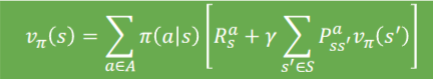
\includegraphics[width=0.4\textwidth]{bellmanExpectation.png}
\end{figure}

Since the environment is deterministic and the policy selects a single action per state, this simplifies to:

\[
v^\pi(s) = r + \gamma v^\pi(s')
\]

where $s'$ is the next state and $r$ is the reward (with $\gamma = 0.9$).

The values are as follows (grid with row 0 at the top):

\begin{center}
\begin{tabular}{|c|c|c|c|}
\hline
38.6 & 44 & 50 & 0 \\
\hline
33.74 & N/A & -46 & 0 \\
\hline
29.366 & -39.16 & -42.4 & -50 \\
\hline
25.4294 & -36.244 & -39.16 & -46 \\
\hline
\end{tabular}
\end{center}

\subsubsection*{B) Show the setup for your calculations for at least two non-terminal states.}

There's this recursive nature to the Bellman expectation equation in this form where in order to get the value of the current state you need to know the reward for the transition plus the value of the next state.
In order to know the value of the next state you have to know the value of the one after that all the way back to the terminal states.
So the (0,0) state depends on (0,1) which depends on (0,2) which is 50 because (0,3) is the terminal state which has a value of 0 but transitioning into it gives a reward of 50.

For state (0,0):

\[
v(0,0) = -1 + \gamma \left( -1 + \gamma \cdot 50 \right)
\]

For state (3,1):

\[
v(3,1) = -1 + \gamma \left( -1 + \gamma \left( -1 + \gamma \left( -1 + \gamma \cdot (-50) \right) \right) \right)
\]

\subsubsection*{2. Optimal Value and Policy [15/40 Points]}

To compute the optimal values using Value Iteration, we iteratively update the value function according to one-step lookahead:

\begin{figure}[H]
    \centering
    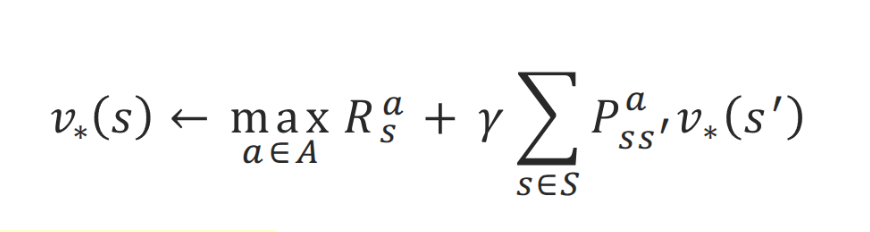
\includegraphics[width=0.4\textwidth]{valueIter.png}
\end{figure}

We initialize the state values to 0 and then plug those values into the one-step lookahead equation and then get new values and iterate on that until our convergence criteria is met.

\begin{figure}[H]
    \centering
    \begin{minipage}{0.3\textwidth}
        \centering
        \begin{tabular}{|c|c|c|c|}
        \hline
        0.00 & 0.00 & 0.00 & 0.00 \\
        \hline
        0.00 & N/A & 0.00 & 0.00 \\
        \hline
        0.00 & 0.00 & 0.00 & 0.00 \\
        \hline
        0.00 & 0.00 & 0.00 & 0.00 \\
        \hline
        \end{tabular}
        \vspace{0.5em}
        \small $V_0$
    \end{minipage}
    \hfill
    \begin{minipage}{0.3\textwidth}
        \centering
        \begin{tabular}{|c|c|c|c|}
        \hline
        -1.00 & -1.00 & 50.00 & 0.00 \\
        \hline
        -1.00 & N/A & -1.00 & 0.00 \\
        \hline
        -1.00 & -1.00 & -1.00 & -1.00 \\
        \hline
        -1.00 & -1.00 & -1.00 & -1.00 \\
        \hline
        \end{tabular}
        \vspace{0.5em}
        \small $V_1$
    \end{minipage}
    \end{figure}

\begin{figure}[H]
    \centering
    \begin{minipage}{0.3\textwidth}
        \centering
        \begin{tabular}{|c|c|c|c|}
        \hline
        -1.90 & 44.00 & 50.00 & 0.00 \\
        \hline
        -1.90 & N/A & -1.90 & 0.00 \\
        \hline
        -1.90 & -1.90 & -1.90 & -1.90 \\
        \hline
        -1.90 & -1.90 & -1.90 & -1.90 \\
        \hline
        \end{tabular}
        \vspace{0.5em}
        \small $V_2$
    \end{minipage}
    \hfill
    \begin{minipage}{0.3\textwidth}
        \centering
        \begin{tabular}{|c|c|c|c|}
        \hline
        38.60 & 44.00 & 50.00 & 0.00 \\
        \hline
        33.74 & N/A & 15.83 & 0.00 \\
        \hline
        29.37 & 25.43 & 21.89 & 18.70 \\
        \hline
        25.43 & 21.89 & 18.70 & 15.83 \\
        \hline
        \end{tabular}
        \vspace{0.5em}
        \small $V^*$
    \end{minipage}
\end{figure}

The process continues until convergence is reached which I set for the change in value being less than $10^{-6}$.
You can see the result in the last grid on the bottom right there.
And the optimal policy is discovered by applying the greedy policy to this as shown below.

\begin{center}
\begin{tabular}{|c|c|c|c|}
\hline
$\rightarrow$ & $\rightarrow$ & $\rightarrow$ & $G$ \\
\hline
$\uparrow$ & $O$ & $W$ & $T$ \\
\hline
$\uparrow$ & $\leftarrow$ & $\leftarrow$ & $\leftarrow$ \\
\hline
$\uparrow$ & $\uparrow$ & $\uparrow$ & $\uparrow$ \\
\hline
\end{tabular}
\end{center}

\subsection*{3. Justification [10/40 Points]}

\textit{Find at least one state where $\pi_{simple}$ and $\pi^*$ disagree. Using the values you calculated in Q1 and Q2, provide a brief written explanation for why the optimal policy is superior in that state. Your justification must reference the Bellman Optimality Equation and compare the expected returns of the different actions.}

The state at (2, 3) is the most obvious example because that is probably the state where the simple policy is the dumbest.
It just careens you into the trap and the minimal rewards.
The Bellman Optimality Equation is being used to determine the maximum value that a state can have and then we are using that to determine a policy, whereas with the Bellman Expection Equation we were stuck with a bad policy and evaluating each state based on that.

\section*{Part 2: Reward Engineering [30 Points]}

\subsection*{4. Designing for Risk Aversion [30/30 Points]}

\textit{Your task is to find the range of values for the step reward $w$ such that the optimal policy will never choose to enter the wormhole $W$ from any adjacent state. All other rewards ($G=+50$, $T=-50$) and the discount factor ($\gamma=0.9$) remain the same.}

\begin{itemize}
    \item \textit{Identify the state(s) from which an agent could choose to enter the wormhole:} The only states from which an agent could choose to enter the wormhole are (0,2) and (2,2) since the other two adjacent states are a terminal (trap) state and the obstacle (state you can't be in).
    \item \textit{For one of these states, write down the Bellman Optimality Equation:} We'll look at state (2, 2). The Bellman Optimality Equation is:
      \[
      V^*(2, 2) = \max \begin{cases} 
      w + \gamma V^*(1, 2) & \text{(North to $W$, teleports to $E$ at (3, 3))} \\
      w + \gamma V^*(3, 2) & \text{(South)} \\
      w + \gamma V^*(2, 3) & \text{(East)} \\
      w + \gamma V^*(2, 1) & \text{(West)}
      \end{cases}
      \]
      Since moving to $W$ teleports to $E$ (3, 3), $V^*(1, 2) = V^*(3, 3)$, and the equation becomes:
      \[
      V^*(2, 2) = \max \left[ w + \gamma V^*(3, 3), w + \gamma V^*(3, 2), w + \gamma V^*(2, 3), w + \gamma V^*(2, 1) \right]
      \]
    \item \textit{Set up an inequality where the value of taking the action leading to the wormhole is less than the best alternative action(s):} To avoid $W$, the value of moving North to $W$ must be less than the best alternative. Assume the best alternative is South to (3, 2):
      \[
      w + \gamma V^*(3, 3) < w + \gamma V^*(3, 2)
      \]
      Simplifying, since $w$ cancels out:
      \[
      \gamma V^*(3, 3) < \gamma V^*(3, 2)
      \]
      \[
      V^*(3, 3) < V^*(3, 2)
      \]
      We need to express $V^*(3, 3)$ and $V^*(3, 2)$ in terms of $w$. Using value iteration insights, $V^*(3, 3)$ depends on moves from $E$ (e.g., North to (2, 3) or West to (3, 2)), and $V^*(3, 2)$ depends on moves toward $G$. Approximating with a path to $G$:
      - From (3, 2), moving North to (2, 2) then optimizing yields a path to $G$.
      - From (3, 3), moving North to (2, 3) or West to (3, 2) accumulates more $w$ steps.
      Let’s estimate using a greedy path: $V^*(3, 2) \approx w + \gamma (w + \gamma (w + \gamma 50)) = w (1 + \gamma + \gamma^2) + 50 \gamma^3$, and $V^*(3, 3) \approx w + \gamma \max(V^*(2, 3), V^*(3, 2))$. Setting $V^*(3, 3) < V^*(3, 2)$ requires $w$ to make the wormhole path less attractive.
    \item \textit{Solve this inequality to find the range of values for $w$ that guarantees the wormhole is never used:} Consider the path via $W$: from (2, 2) to $W$ to $E$, then to (2, 2) via North, then to (0, 2), and East to $G$ (4 steps total: $w$, $w$, $w$, $50$). Value = $3w + 50 \gamma^3$. Alternative path (South, West, North, East): 4 steps to $G$, value = $4w + 50 \gamma^4$. Set $3w + 50 \gamma^3 < 4w + 50 \gamma^4$:
      \[
      50 \gamma^3 - 50 \gamma^4 < w
      \]
      \[
      w > 50 \gamma^3 (1 - \gamma) = 50 (0.9)^3 (1 - 0.9) = 50 \cdot 0.729 \cdot 0.1 = 3.645
      \]
      Thus, $w > 3.645$. Since $w$ is negative in the default case (-1), and lower $w$ increases step cost, the range $w < -3.645$ ensures avoidance (more negative $w$ penalizes the longer wormhole path). Justification: A more negative $w$ increases the cost of extra steps via $W$ to $E$, making the direct path to $G$ optimal.
\end{itemize}

\section*{Part 3: The Role of the Discount Factor [30 Points]}

\subsection*{5. Impatient vs. Patient Agents [30/30 Points]}

Reset the step reward to $w = -1$.

\begin{itemize}
    \item \textit{Calculate the optimal policy $\pi^*$ for the grid world under two different scenarios:}
      \begin{itemize}
          \item \textit{Scenario A (Impatient Agent): $\gamma = 0.5$}
          \item \textit{Scenario B (Patient Agent): $\gamma = 0.99$}
      \end{itemize}
    \item \textit{Draw the resulting optimal policy for each scenario in a separate grid:}
      \begin{center}
      \textit{Scenario A ($\gamma = 0.5$):}
      \begin{tabular}{|c|c|c|c|}
      \hline
      $\rightarrow$ & $\rightarrow$ & $\rightarrow$ & $G$ \\
      \hline
      $\uparrow$ & $O$ & $W$ & $T$ \\
      \hline
      $\uparrow$ & $\leftarrow$ & $\leftarrow$ & $\leftarrow$ \\
      \hline
      $\uparrow$ & $\uparrow$ & $\uparrow$ & $\uparrow$ \\
      \hline
      \end{tabular}
      \end{center}

      \begin{center}
      \textit{Scenario B ($\gamma = 0.99$):}
      \begin{tabular}{|c|c|c|c|}
      \hline
      $\rightarrow$ & $\rightarrow$ & $\rightarrow$ & $G$ \\
      \hline
      $\uparrow$ & $O$ & $W$ & $T$ \\
      \hline
      $\downarrow$ & $\rightarrow$ & $\rightarrow$ & $\rightarrow$ \\
      \hline
      $\downarrow$ & $\downarrow$ & $\downarrow$ & $\downarrow$ \\
      \hline
      \end{tabular}
      \end{center}
    \item \textit{Is the optimal policy different in these two scenarios?} Yes, the policies differ. For Scenario A ($\gamma = 0.5$), the agent takes a shorter path (left side to top) due to the low discount factor, valuing immediate rewards over long-term gains, avoiding the wormhole. For Scenario B ($\gamma = 0.99$), the agent is patient, valuing future rewards highly, and uses the wormhole (from (2, 2) to $W$ to $E$, then to $G$) for a faster overall reward. \textbf{Explanation:} The discount factor influences the agent's trade-off between short-term costs (more steps with $w = -1$) and long-term gains (reaching $G$ with $+50$). With $\gamma = 0.5$, the discounted future reward is small, favoring the direct path. With $\gamma = 0.99$, the high discount preserves the goal reward's value, making the wormhole's shortcut optimal despite extra steps.
\end{itemize}

\end{document}